\documentclass{article}
\usepackage{tikz}
\usepackage{amsmath,amssymb}
\begin{document}

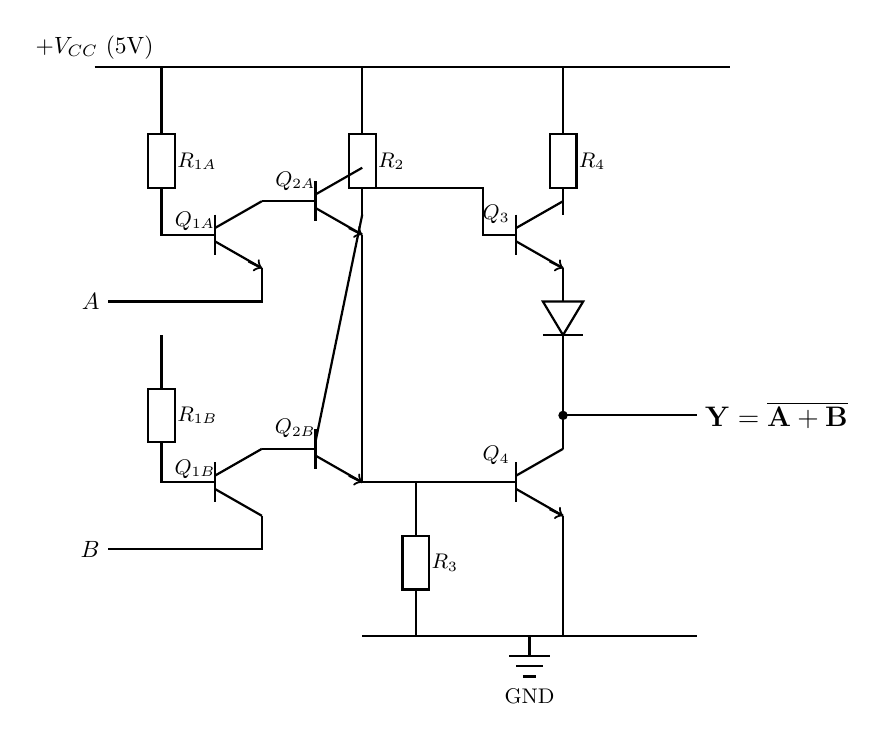
\begin{tikzpicture}[scale=0.85, transform shape]
  % VCC Rail
  \draw[thick] (-1.0, 6.0) -- (8.5, 6.0);
  \node at (-1.0, 6.3) {$+V_{CC}\ (5\text{V})$};

  % Resistors to VCC
  % R1A (4k)
  \draw[thick] (0, 6.0) -- (0, 5.0);
  \draw[thick] (-0.2, 5.0) rectangle (0.2, 4.2) node[midway, right=3pt]{\small $R_{1A}$};
  \draw[thick] (0, 4.2) -- (0, 3.5) -- (0.8, 3.5);

  % Q1A Input Transistor
  \draw[thick] (0.8, 3.8) -- (0.8, 3.2); % Base bar
  \draw[thick] (0.8, 3.6) -- (1.5, 4.0); % Collector to Q2A Base
  \draw[thick] (0.8, 3.4) -- (1.5, 3.0); % Emitter
  \draw[thick, ->] (1.3, 3.1) -- (1.5, 3.0); % Emitter arrow (pointing in for multi-emitter or out)
  \draw[thick] (1.5, 3.0) -- (1.5, 2.5) -- (-0.8, 2.5);
  \node[left] at (-0.8, 2.5) {$A$};
  \node at (0.5, 3.7) {\small $Q_{1A}$};

  % Q1B Input Transistor (Lower)
  \draw[thick] (0, 2.0) -- (0, 1.2);
  \draw[thick] (-0.2, 1.2) rectangle (0.2, 0.4) node[midway, right=3pt]{\small $R_{1B}$};
  \draw[thick] (0, 0.4) -- (0, -0.2) -- (0.8, -0.2);

  \draw[thick] (0.8, 0.1) -- (0.8, -0.5);
  \draw[thick] (0.8, -0.1) -- (1.5, 0.3); % Collector to Q2B Base
  \draw[thick] (0.8, -0.3) -- (1.5, -0.7); % Emitter
  \draw[thick] (1.5, -0.7) -- (1.5, -1.2) -- (-0.8, -1.2);
  \node[left] at (-0.8, -1.2) {$B$};
  \node at (0.5, 0.0) {\small $Q_{1B}$};

  % Phase Splitters Q2A & Q2B (in parallel)
  \draw[thick] (3.0, 6.0) -- (3.0, 5.0);
  \draw[thick] (2.8, 5.0) rectangle (3.2, 4.2) node[midway, right=3pt]{\small $R_2$};
  \draw[thick] (3.0, 4.2) -- (3.0, 3.8);

  % Q2A
  \draw[thick] (1.5, 4.0) -- (2.3, 4.0);
  \draw[thick] (2.3, 4.3) -- (2.3, 3.7);
  \draw[thick] (2.3, 4.1) -- (3.0, 4.5); % Coll
  \draw[thick] (2.3, 3.9) -- (3.0, 3.5); % Emit
  \draw[thick, ->] (2.8, 3.6) -- (3.0, 3.5);
  \node at (2.0, 4.3) {\small $Q_{2A}$};

  % Q2B
  \draw[thick] (1.5, 0.3) -- (2.3, 0.3);
  \draw[thick] (2.3, 0.6) -- (2.3, 0.0);
  \draw[thick] (2.3, 0.4) -- (3.0, 3.8); % Parallel Collector tied together
  \draw[thick] (2.3, 0.2) -- (3.0, -0.2); % Emit
  \draw[thick, ->] (2.8, -0.1) -- (3.0, -0.2);
  \node at (2.0, 0.6) {\small $Q_{2B}$};

  % Combined Emitters to R3 and Q4 Base
  \draw[thick] (3.0, 3.5) -- (3.0, -0.2) -- (3.8, -0.2);
  \draw[thick] (3.8, -0.2) -- (3.8, -1.0);
  \draw[thick] (3.6, -1.0) rectangle (4.0, -1.8) node[midway, right=3pt]{\small $R_3$};
  \draw[thick] (3.8, -1.8) -- (3.8, -2.5);

  % Totem Pole Pull-Up Q3
  \draw[thick] (6.0, 6.0) -- (6.0, 5.0);
  \draw[thick] (5.8, 5.0) rectangle (6.2, 4.2) node[midway, right=3pt]{\small $R_4$};
  \draw[thick] (6.0, 4.2) -- (6.0, 3.8);

  \draw[thick] (3.0, 4.2) -- (4.8, 4.2) -- (4.8, 3.5) -- (5.3, 3.5);
  \draw[thick] (5.3, 3.8) -- (5.3, 3.2);
  \draw[thick] (5.3, 3.6) -- (6.0, 4.0); % Coll
  \draw[thick] (5.3, 3.4) -- (6.0, 3.0); % Emit
  \draw[thick, ->] (5.8, 3.1) -- (6.0, 3.0);
  \node at (5.0, 3.8) {\small $Q_3$};

  % Diode D1
  \draw[thick] (6.0, 3.0) -- (6.0, 2.5);
  \draw[thick] (5.7, 2.5) -- (6.3, 2.5) -- (6.0, 2.0) -- cycle; % Diode triangle
  \draw[thick] (5.7, 2.0) -- (6.3, 2.0); % Diode bar
  \draw[thick] (6.0, 2.0) -- (6.0, 1.2);

  % Totem Pole Pull-Down Q4
  \draw[thick] (3.8, -0.2) -- (5.3, -0.2);
  \draw[thick] (5.3, 0.1) -- (5.3, -0.5);
  \draw[thick] (5.3, -0.1) -- (6.0, 0.3); % Coll
  \draw[thick] (5.3, -0.3) -- (6.0, -0.7); % Emit
  \draw[thick, ->] (5.8, -0.6) -- (6.0, -0.7);
  \node at (5.0, 0.2) {\small $Q_4$};

  % Output Node
  \draw[thick] (6.0, 1.2) -- (6.0, 0.3);
  \draw[thick] (6.0, 0.8) -- (8.0, 0.8);
  \node[right] at (8.0, 0.8) {\large $\mathbf{Y = \overline{A + B}}$};
  \fill (6.0, 0.8) circle (2pt);

  % Ground Rail
  \draw[thick] (6.0, -0.7) -- (6.0, -2.5) -- (3.0, -2.5) -- (8.0, -2.5);
  \draw[thick] (5.5, -2.5) -- (5.5, -2.8);
  \draw[thick] (5.2, -2.8) -- (5.8, -2.8);
  \draw[thick] (5.3, -2.95) -- (5.7, -2.95);
  \draw[thick] (5.4, -3.1) -- (5.6, -3.1);
  \node at (5.5, -3.4) {\small GND};
\end{tikzpicture}

\end{document}
